%! Author = mariuszindel
%! Date = 02.11.20

\section{LINQ}


\subsection{Überblick}
Sprach-integrierte Abfragesprache:
\begin{itemize}
    \item Reine Compiler-Technologie
    \item Query-Syntax (ähnlich SQL)
    \item Beliebige Datenstrukturen als Basis
    \item Typensicherheit
    \item Erlaubt «Funktionale Programmierung» mittels «Lambda Expressions»
    \item Erlaubt «Deklarativen Programmierstil» mittels «Anonymous Types» und «Object Initializers»
\end{itemize}
\subsubsection{Architektur}
\begin{center}
    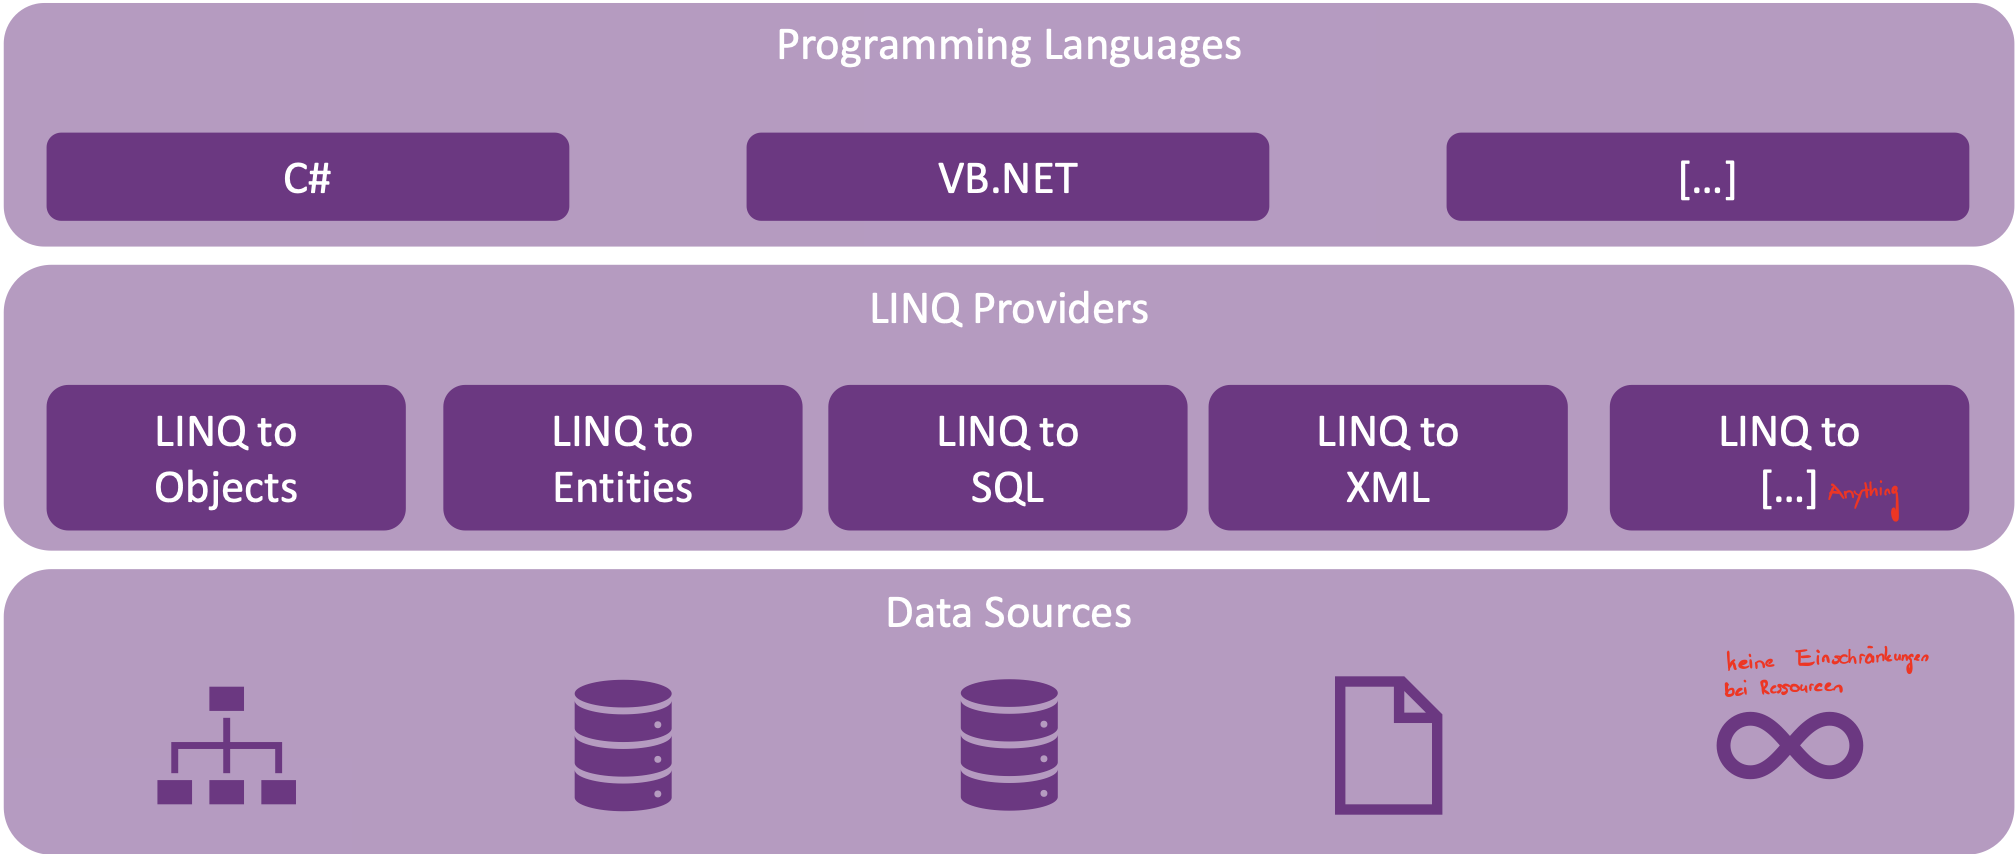
\includegraphics[scale=.2]{graphic/linq/Architektur.png}
\end{center}
\vspace{-8pt}

\subsubsection{Beispiel}
\begin{itemize}
    \item  Abfrage auf Objektstruktur
    \item Query / Lambda Expression 1
    \begin{itemize}
        \item Reine Selektion (ganzes Objekt)
    \end{itemize}
    \item Query / Lambda Expression 2
    \begin{itemize}
        \item Filter nach Namen beginnend mit «B»
        \item Sortierung
        \item Selektion (ganzes Objekt)
    \end{itemize}
    \item Query Expressions werden vom Compiler in Lamda Expressions umgewandelt
\end{itemize}
\vspace{-8pt}
\begin{center}
    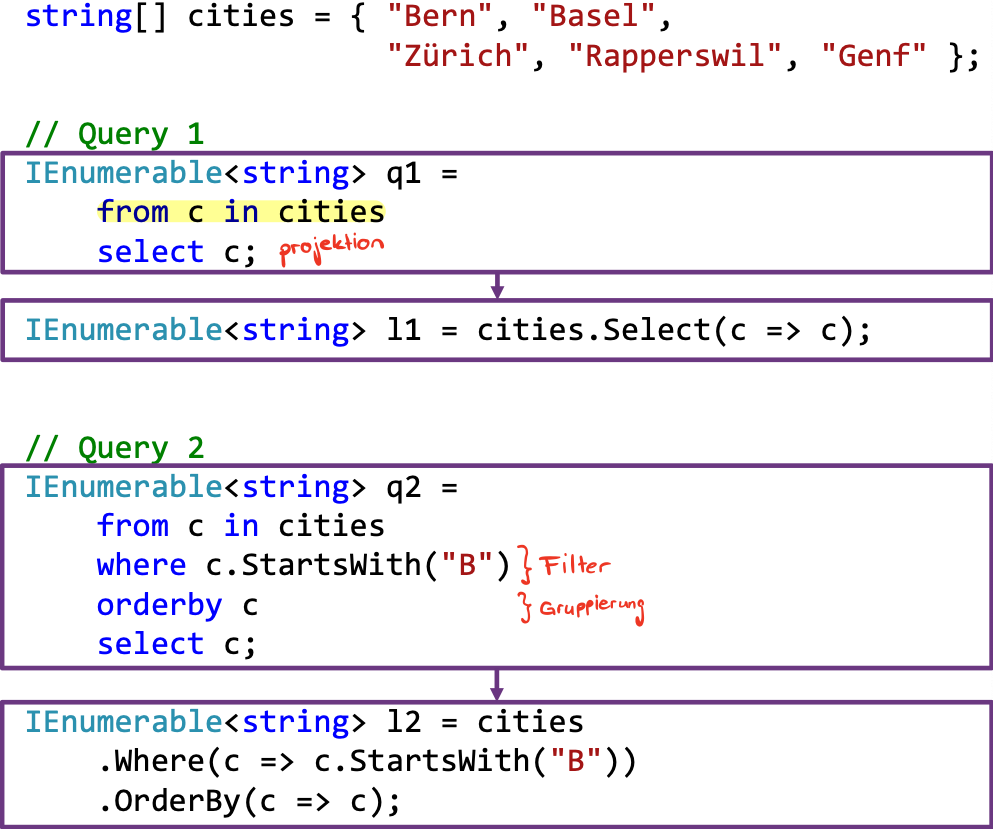
\includegraphics[scale=.35]{graphic/linq/Beispiel LINQ to Objects.png}
\end{center}
\vspace{-8pt}

\subsubsection{Syntax}
\begin{lstlisting}
IEnumerable<string> q2 =
    from c in cities
    where c.StartsWith("B")
    orderby c
    select c;
\end{lstlisting}


\subsection{Lambda Expressions}
\subsubsection{Überblick}
\begin{itemize}
    \item Eine Lambda Expression ist eine Anonyme Methode
    \begin{itemize}
        \item Keine Implementation einer benannten Methode nötig
        \item Kein «delegate» Schlüsselwort mehr nötig
        \item Angabe von Parametertypen optional
    \end{itemize}
    \item Basis für das Erzeugen von
    \begin{itemize}
        \item Delegates
        \item Expression Trees
    \end{itemize}
    \item Zwei Ausprägungen
    \begin{itemize}
        \item Expression Lambdas\\
        («parameters») => expression
        \item Statement Lambdas\\
        («parameters») => { statements; }
    \end{itemize}
\end{itemize}

\begin{lstlisting}
// Expression Lambda
Func<int, bool> fe = i => i % 2 == 0;

// Statement Lambda
Func<int, bool> fs = i => {
    int rest = i%2;
    bool isRestZero = rest == 0;
    return isRestZero;
};
\end{lstlisting}

\subsubsection{Parameter}
\begin{itemize}
    \item Lambdas können 0 – n Parameter haben
    \item Typ-Definition kann oftmals weggelassen werden
    \item Regeln:
    \begin{itemize}
        \item Klammern um Parameter-Definition
        \item «ref» und «out» Parameter sind erlaubt
        \item Jeder Parameter muss implizit in den jeweiligen Delegate-Parameter konvertierbar sein
    \end{itemize}
\end{itemize}
\begin{lstlisting}
Func<bool> p01;
Func<int, bool> p02;
Func<int, int, bool> p03;
Func<int, int, int, bool> p04;

p01 = () => true;          // 0 Parameters
p02 = a => true;           // 1 Parameter
p02 = (a) => true;         // 1 Parameter
p03 = (a, b) => true;      // 2 Parameters
p04 = (a, b, c) => true;   // 3 Parameters // ...

p01 = () => true;                    // 0 Parameters
p02 = int a => true;                 // Compilerfehler
p02 = (int a) => true;               // 1 Parameter
p03 = (int a, int b) => true;        // 2 Parameters
p04 = (int a, int b, int c) => true; // 3 Parameters
\end{lstlisting}

\subsubsection{Type Inference}
\begin{itemize}
    \item Parametertypen sind meist redundant definiert
    \item Somit ist Angabe in Parameterliste obsolet
\end{itemize}
\vspace{-8pt}
\begin{center}
    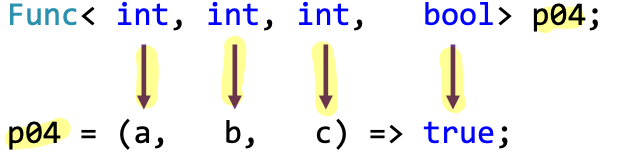
\includegraphics[scale=.33]{graphic/linq/Type Inference.png}
\end{center}
\vspace{-8pt}

\subsubsection{Expression Lambdas}
Syntax:
\begin{lstlisting}
(parameters) => expression

Func<int, int> e1;
e1 = a => a * a;
\end{lstlisting}


\subsubsection{Statement Lambdas}
Syntax:
\begin{lstlisting}
(parameters) => { statements; }

Func<int, int> e1;
e1 = a => { return a * a; };
\end{lstlisting}

\subsubsection{Variable Scope}
Regeln:
\begin{itemize}
    \item Lambda Expression kann auf äussere Variablen zugreifen
    \item Variablen in Lamda Expressions sind für äussere Methoden nicht sichtbar
    \item Zugriff auf «out» und «ref» Parameter nicht erlaubt
\end{itemize}
\begin{lstlisting}
public void TestOuterVariables() {
    int x = 0;
    Action a = () => x = 1;

    Console.WriteLine(x); // Output: 0
    a();
    Console.WriteLine(x); // Output: 1
\end{lstlisting}


\subsection{LINQ Extension Methods}

\subsubsection{Überblick}
\begin{itemize}
    \item LINQ definiert in der Klasse Enumerable eine Vielzahl von Query Operatoren
    \item  Die Methoden in dieser Klasse stellen eine Implementierung von Operatoren zum Abfragen von Datenquellen bereit, die IEnumerable<T> implementieren.
\end{itemize}
\begin{lstlisting}
using System.Linq;

int[] numbers = { 1, 4, 2, 9, 13, 8, 9, 0, -6, 12 };

IEnumerable<int> res = numbers
    .Where(i => i >= 5)
    .OrderBy(i => i);

IEnumerable<int> sqr = numbers
    .Skip(2)
    .Take(4)
    .Select(k=> k * k);
\end{lstlisting}

\subsubsection{Deferred Evaluation}
\begin{itemize}
    \item Query Operatoren sind ebenfalls mit «yield return» implementiert
    \item Queries können beliebig oft ausgeführt werden
\end{itemize}

\subsubsection{Immediate Evaluation}
Einige Operatoren führen Queries direkt aus $\rightarrow$ Wenn Rückgabewert nicht «IEnumerable» ist:
\begin{itemize}
    \item ToList / ToArray
    \item Count / First
    \item Sum / Average
    \item etc.

\end{itemize}
\begin{lstlisting}
public void TestDeferredEvaluation() {

string[] cities = { "Bern", "Basel", "Zuerich", "Rapperswil", "Genf" };

// Ausfuehrung
List<string> citiesB = cities
    .Where(c => c.StartsWith("B"))
    .ToList();

// Ausfuehrung
int citiesEndL = cities
    .Where(c => c.EndsWith("l"))
    .Count();}
\end{lstlisting}


\subsection{Expression-bodied Members}
\begin{itemize}
    \item Allgemein
    \begin{itemize}
        \item Lambda-Expression anstelle von Block { }
        \item Darf aus maximal einem Statement bestehen
    \end{itemize}
    \item Funktioniert für
    \begin{itemize}
        \item Methoden / Operatoren
        \item Konstruktoren / Destruktoren
        \item Properties / Indexers
    \end{itemize}
    \item Spezialfall «Properties»
    \begin{itemize}
        \item Read-Only Properties brauchen keinen Statement-Block { }
        \item Get/Set- und reine Set-Properties schon
    \end{itemize}
\end{itemize}


\subsection{Object / Collection Initializers}

\subsubsection{Object Initializers}
\begin{itemize}
    \item Erlaubt das Instanzieren und Initialisieren einer Klasse in einem Statement
    \item  Reine Compiler-Technologie
\end{itemize}
\begin{lstlisting}
class Student {
    public string Name;
    public int Id;
    public string Subject { get; set; }
    public Student() { }
    public Student(string name) { Name = name; }
}

class Examples {
    public void Test() {
        Student s1 = new Student("John") {
            Id = 2009001, // Set public field
            Subject = "Computing" // Set property
        };
        int[] ids = { 2009001, 2009002, 2009003 };
        IEnumerable<Student> students = ids
            .Select(n => new Student { Id = n });}
}}
\end{lstlisting}

\subsubsection{Collection Initializers (Collections)}
Erlaubt das Instanzieren und Initialisieren einer Collection in einem Statement:
\begin{lstlisting}
//Syntax:
new collection
{ elem1 , ..., elemN };

//Bsp:
class Examples {
public void Test() {
    List<int> l1 = new List<int>
        { 1, 2, 3, 4 }
\end{lstlisting}

\subsubsection{Collection Initializers (Dictionaries)}
Erlaubt das Instanzieren und Initialisieren eines Dictionaries in einem Statement:
\begin{lstlisting}
//Syntax:
new dictionary
{ { key1, v1 }, ...,
    { keyN, vN } };

//Bsp:
class Examples {
    public void Test() {
        Dictionary<int, string> d1 = new Dictionary<int, string>
            {
                { 1, "a" },
                { 2, "b" },
                { 3, "c" }
            };
    }}
\end{lstlisting}

\subsubsection{Kombination}
\begin{itemize}
    \item Object und Collection Initializers lassen sich beliebig kombinieren
    \item Wird oft auch für GUI-Aufbau oder Test-Datenstrukturen verwendet
\end{itemize}
\begin{lstlisting}
object s = new Dictionary<int, Student> {

{ 2009001, new Student("John") {
    Id = 2009001, Subject = "Computing" } },

{ 2009002, new Student {
    Name = "Ann", Id = 2009002, Subject = "Mathematics" } }
};
\end{lstlisting}


\subsection{Anonymous Types}

\subsubsection{Schlüsselwort «var» / Type Inference}
\begin{itemize}
    \item Typ einer Variable muss nicht mehr angegeben
    \item «var» wird anstelle des Typen verwendet
    \item Deklaration und Initialisierung müssen im gleichen Statement sein
    \item Schlüsselwort «var»
    \begin{itemize}
        \item wird vom Compiler durch korrekten Typen ersetzt
        \item kann nur für lokale Variablen verwendet werden
        \item kann nicht als Parameter, Klassen-Variable, Property-Typ, etc.
    \end{itemize}
    \item Im IL-Code steht der effektive Typ
\end{itemize}

\subsubsection{Überblick}
\begin{itemize}
    \item Erzeugung eines Strukturierten Wertes
    \item Meist in LINQ Queries verwendet (Projektion)
\end{itemize}

\subsubsection{Syntax}
\begin{lstlisting}
var a = new { Id = 1, Name = "John" };
var b = new { a.Id, a.Name };
\end{lstlisting}




\section{LINQ Query Expressions}

\subsection{Einführung}
\subsubsection{Überblick}
\begin{itemize}
    \item SQL-ähnliche Syntax
    \item Bestandteile einer Query Operation
    \begin{itemize}
        \item Datenquelle wählen 
        \item Query definieren 
        \item Query gegen Datenquelle ausführen
    \end{itemize}
\end{itemize}
\begin{lstlisting}
// 1. Datenquelle waehlen
int[] numbers = { 0, 1, 2, 3, 4, 5, 6 };

// 2. Query erstellen
var numQuery =
    from num in numbers
    where (num % 2) == 0
    select num;

// 3. Query ausfuehren
foreach (int num in numQuery) {
    Console.Write("{0,1} ", num);
}
\end{lstlisting}

\subsubsection{Query Syntax}
7 Query-Schlüsselwörter:
\begin{enumerate}
    \item from: Definiert eine Range-Variable und eine Datenquelle
    \item where: Filter
    \item orderby: Sortierung
    \item select: Projektion auf einen Elementtypen
    \item group: Gruppierung in eine Sequenz von Gruppen-Elementen 
    \item join: Verknüpfung zweier Datenquellen
    \item let: Definition von Hilfsvariablen
\end{enumerate}
\begin{lstlisting}
var q1 = from s in Students
    where s.Subject == "Computing"
    orderby s.Name
    select new { s.Id, s.Name };
\end{lstlisting}
\begin{itemize}
    \item beginnt immer mit «from»
    \item endet immer mit «select» oder «group»
\end{itemize}

\subsection{Abfragen}
\subsubsection{Query Operatoren / Extension Methoden}
\begin{center}
    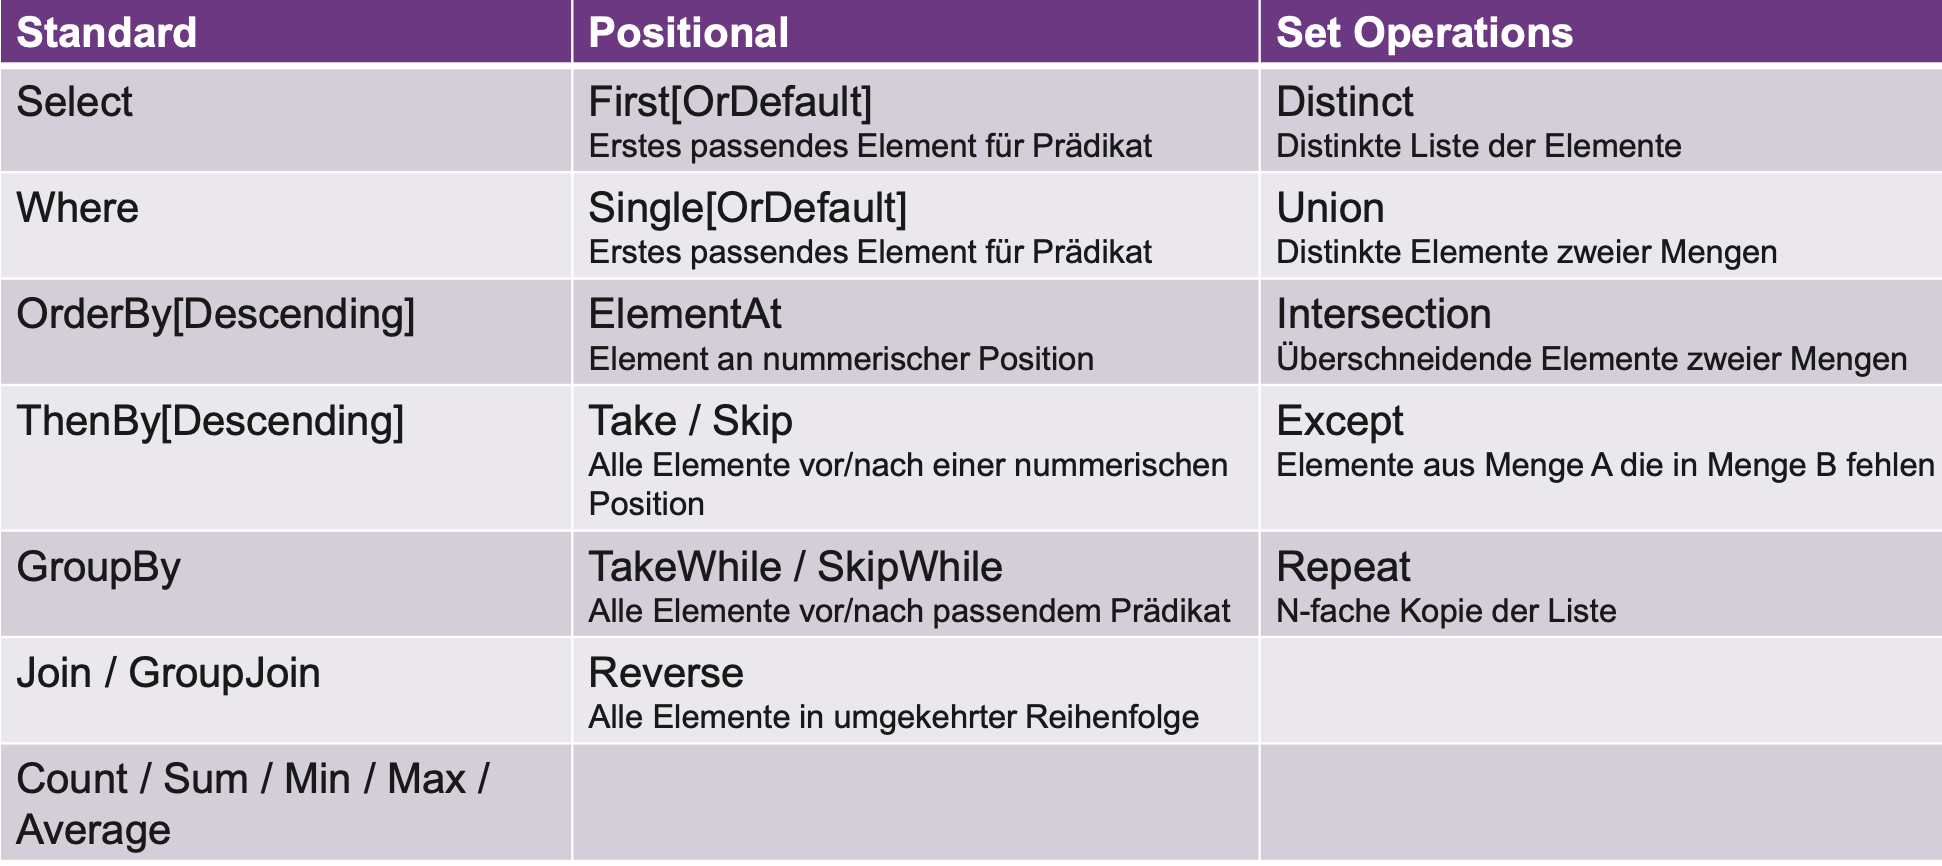
\includegraphics[width=\linewidth]{graphic/linq/Query Operatoren.png}
\end{center}
\vspace{-8pt}

\subsubsection{Range Variablen}
\begin{itemize}
    \item Enstehen durch folgende Klauseln:
    \begin{itemize}
        \item from
        \item join
        \item into
    \end{itemize}
    \item Sind «readonly»
\end{itemize}
\vspace{-8pt}
\subsubsection{Query Operatoren / Extension Methoden}
\begin{center}
    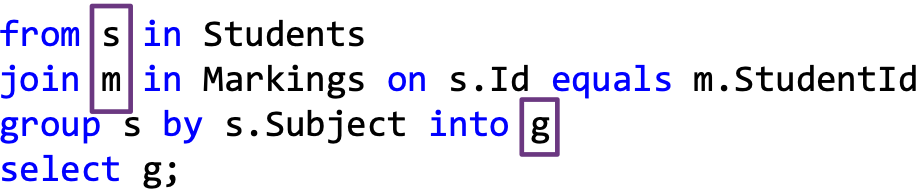
\includegraphics[scale=.3]{graphic/linq/Range Variablen.png}
\end{center}
\vspace{-8pt}

\subsubsection{Gruppierung}
\begin{itemize}
    \item Transformation in «Key/Value Pairs»
    \item Zusammenfassung in ein IEnumerable der Gruppen nach «Key»
\end{itemize}
\vspace{-8pt}
\begin{center}
    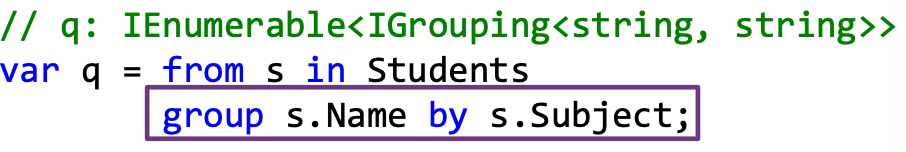
\includegraphics[scale=.3]{graphic/linq/Gruppierung.png}
\end{center}
\vspace{-8pt}

\subsubsection{Gruppierung / Direkte Weiterverwendung}
«into» speichert Resultat in Variable «g»
\begin{itemize}
    \item «s» ist danach nicht mehr sichbar
    \item «g» kann als Gruppe weiterverwendet werden
\end{itemize}
\vspace{-8pt}
\begin{center}
    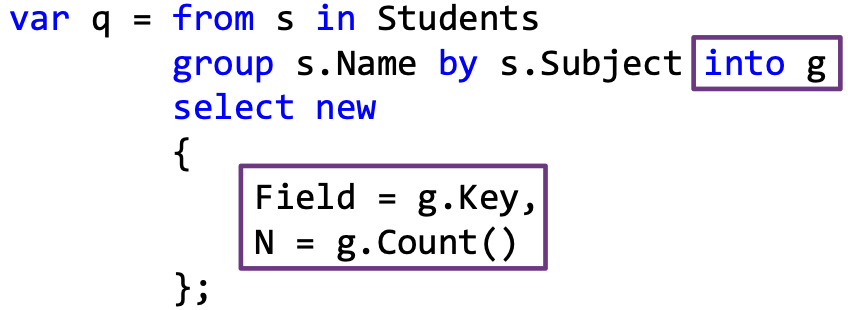
\includegraphics[scale=.3]{graphic/linq/Gruppierung Direkte Weiterverwendung.png}
\end{center}
\vspace{-8pt}

\subsubsection{Inner Joins / Explizit}
\begin{itemize}
    \item Verknüpft zwei Mengen über einen Schlüssel
    \item Zwingend mit «equals» verknüpfen (nicht mit ==)
\end{itemize}
\vspace{-8pt}
\begin{center}
    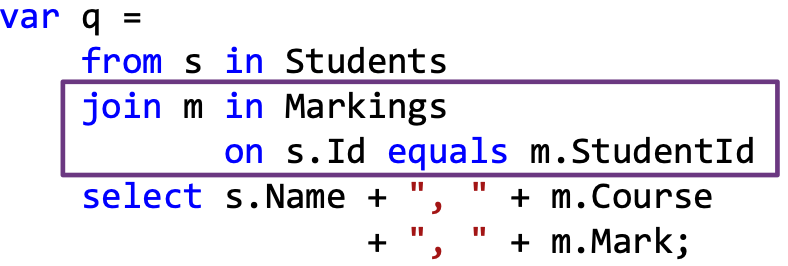
\includegraphics[scale=.3]{graphic/linq/inner join.png}
\end{center}
\vspace{-8pt}

\subsubsection{Inner Joins / Implizit}
\begin{itemize}
    \item Verknüpft zwei Mengen über einen Schlüssel
    \item Unterschied: Weniger effizient
    \begin{itemize}
        \item Bildet Kreuzprodukt
        \item Reduziert Kreuzprodukt bei zutreffender «where» Klausel
    \end{itemize}
\end{itemize}
\vspace{-8pt}
\begin{center}
    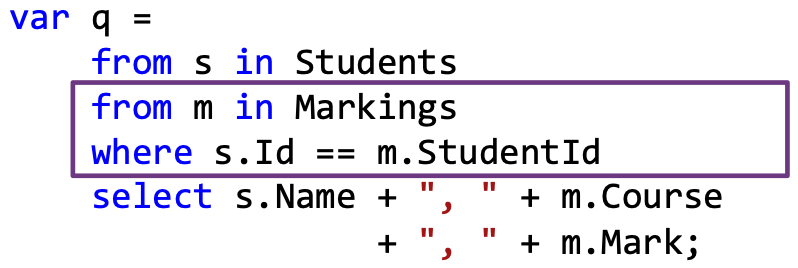
\includegraphics[scale=.3]{graphic/linq/inner join implizit.png}
\end{center}
\vspace{-8pt}

\subsubsection{Group Joins}
\begin{itemize}
    \item Pro «Student» wird eine Liste für alle «Markings» erstellt
    \item «s» bleibt sichtbar
\end{itemize}
\vspace{-8pt}
\begin{center}
    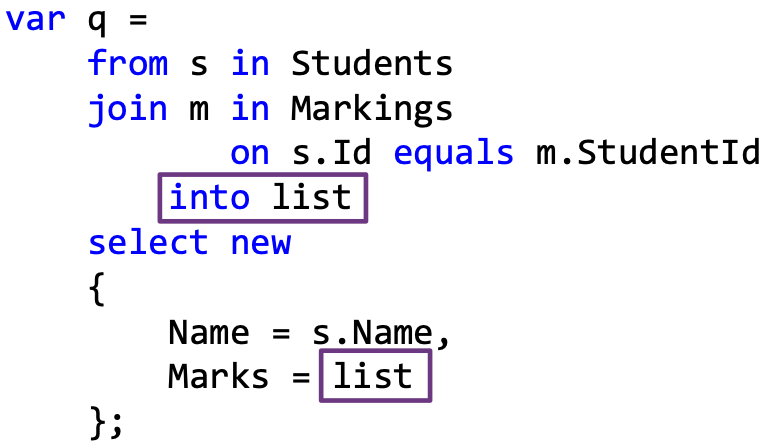
\includegraphics[scale=.3]{graphic/linq/Group Joins.png}
\end{center}
\vspace{-8pt}

\subsubsection{Left Outer Joins}
\begin{itemize}
    \item Verknüpft zwei Mengen über einen Schlüssel
    \item Wenn kein rechtes Element gefunden wird bleibt linkes Element trotzdem bestehen
\end{itemize}
\vspace{-8pt}
\begin{center}
    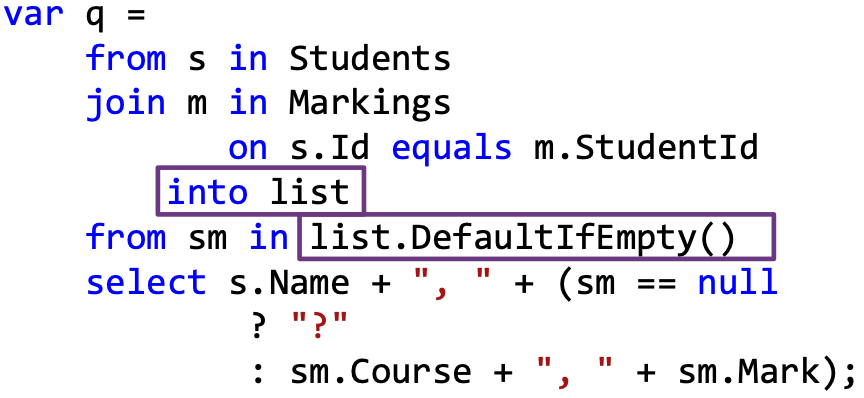
\includegraphics[scale=.3]{graphic/linq/Left Outer Joins.png}
\end{center}
\vspace{-8pt}

\subsubsection{let Klausel}
\begin{itemize}
    \item Erlaubt das Definieren von Hilfsvariablen
\end{itemize}
\vspace{-8pt}
\begin{center}
    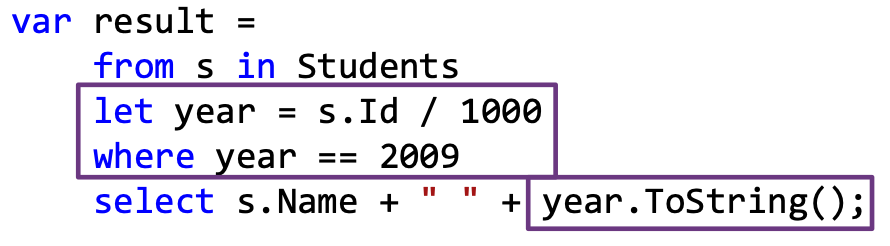
\includegraphics[scale=.3]{graphic/linq/let Klausel.png}
\end{center}
\vspace{-8pt}

\subsubsection{Select Many}
\begin{itemize}
    \item Erleichtert das zusammenfassen verschachtelter Listen
    \item Für jedes Listenelement auf oberster Stufe den «selector» aus
    \item Dieser liefert selbst eine Liste (Teilliste)
    \item Teillisten werden untereinander gehängt
\end{itemize}
\vspace{-8pt}
\begin{center}
    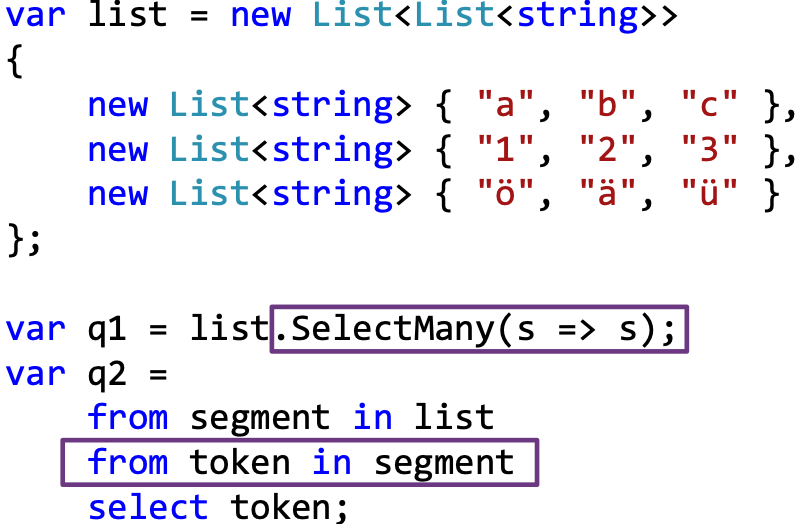
\includegraphics[scale=.3]{graphic/linq/Select Many.png}
\end{center}
\vspace{-8pt}


\newpage